\documentclass[a4paper,12pt]{article} % добавить leqno в [] для нумерации слева
\usepackage[a4paper,top=1.3cm,bottom=2cm,left=1.5cm,right=1.5cm,marginparwidth=0.75cm]{geometry}

\usepackage[warn]{mathtext}
\usepackage[T2A]{fontenc}
\usepackage[utf8]{inputenc} 
\usepackage[english, russian]{babel}

\usepackage{ upgreek }
\usepackage[table,xcdraw]{xcolor}

\usepackage{indentfirst} %tabutation

\usepackage{amsmath, amsfonts, amssymb, amsthm, mathtools, mathtext} 

\usepackage{graphicx}

\usepackage{wrapfig}
\usepackage{tabularx}

\usepackage{graphicx}%Вставка картинок правильная
\usepackage{float}%"Плавающие" картинки
\usepackage{wrapfig}% Обтекание фигур (таблиц, картинок и прочего)

%%% Дополнительная работа с математикой
\usepackage{amsmath,amsfonts,amssymb,amsthm,mathtools} % AMS





%%% Заголовок
\author{Устюжанина Мария Алексеевна}
\title{Лабораторная работа №1.2.3
Отчет о выполнении лабораторной работы 1.2.
}
\date{\today}

\begin{document}

\begin{titlepage}
	\begin{center}
		{\large МОСКОВСКИЙ ФИЗИКО-ТЕХНИЧЕСКИЙ ИНСТИТУТ (НАЦИОНАЛЬНЫЙ ИССЛЕДОВАТЕЛЬСКИЙ УНИВЕРСИТЕТ)}
	\end{center}
	\begin{center}
		{\large Физтех-школа радиотехники и кибернетики.}
	\end{center}
	
	
	\vspace{4.5cm}
	{\huge
		\begin{center}
			{\bf Отчёт о выполнении лабораторной работы 1.2.3}\\
			 Определение моментов инерции твердых тел с помощью трифилярного подвеса.
		\end{center}
	}
	\vspace{2cm}
	\begin{flushright}
		{\LARGE Автор:\\ Устюжанина Мария Алексеевна \\
			\vspace{0.2cm}
			Б01-107}
	\end{flushright}
	\vspace{8cm}
	\begin{center}
		Долгопрудный 2021
	\end{center}
\end{titlepage}

\section*{Введение}

\textbf{Цель работы:}

	Измерение момента инерции тела и сравнение результатов с расчетами по теоретическим формулам. Проверка аддитивности моментов инерции и справедливости формулы Гюйгенса-Штейнера.

\textbf{Идея:}
     В эксперименте используется связь между периодом колебаний крутильного маятника и его моментом инерции. В качестве маятника используется трифилярный подвес, круглая платформа, подвешенная в поле тяжести на трех длинных нитях. Платформа может совершать крутильные колебания вокруг вертикальной оси. На платформу помещаются тела различной формы, измеряются периоды колебаний маятника и определяются значения моментов инерции этих тел. Теорема Гюйгенса-Штейнера проверяется по соответствию между экспериментальной и теоретической зависимостями моментов инерции грузов от их расстояния до центра платформы.

\medskip

\textbf{В работе используются:} Трифилярный подвес, секундомер, счетчик числа колебаний, набор тел, момент инерции которых необходимо измерить.

\medskip



\section{Теоретические данные.}

\begin{figure}[h]
\center{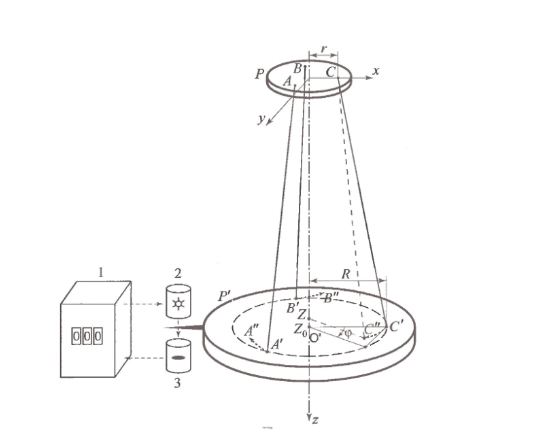
\includegraphics[scale=1.2]{Рис1}}
\caption{Трифилярный подвес}
\label{fig:image}
\end{figure}

	Перед началом работы кратко изложим теоретический материал, связанный с данной темой.

	
	Формула для нахождения момента инерции твердого тела отноcительно неподвижной оси вращения:

	\begin{equation}
			I = \int r^2 dm, 
			 \label{equ:iner}	
	\end{equation}

	где r - расстояние элемента массы тела dm от оси вращения. Интегрирование производиться по всей массе тела.

		
	Уравнение сохранения энергии при колебаниях:

			\[ \frac{I\ddot{\phi}^2}{2} + mg(z_{0} - z) = E \]


			\[ (R\cos\phi - r)^2 + R^2\sin^2\phi + z^2 = L^2  \]

		
			\[ z^2 = L^2 - R^2 - r^2 + 2Rr\cos\phi \approx z^2_{0} - 2Rr(1 - \cos\phi) \approx z^2_{0} - Rr\phi^2 \]


			\[ z = \sqrt{z^2_{0} - Rr\phi^2} \approx z_{0} - \frac{Rr\phi^2}{2z_{0}}\]
			

		Трифилярный подвес состоит из укрепленной на некоторой высоте 				неподвижной 	платформе P и подвешенной к ней на трех симметрично расположенных нитях $ AA', BB', CC' $ вращающейся платформы P'.
	
		Подставляя данное уравнение в уравнение Закона Сохранения Энергии и дважды дифференцируя по 				времени, после сокращений, получаем:
		
	\begin{equation}
		 I\ddot{\phi}^2 + mg\frac{Rr}{z_{0}}\phi = 0 
		 \label{equ:first}	
	\end{equation}
	
	
		Решая уравнение (\ref{equ:first}) относительно $\phi$, получаем:
			
	
	\begin{equation}
		\phi = \phi_{0}\sin\left(\sqrt{\frac{mgRr}{Iz_{0}}}t + \theta\right)
		\label{equ:second}
	\end{equation}
	
	
	Из (\ref{equ:second}) следует, что 
	
	\begin{equation}
		T = 2\pi\sqrt{\frac{Iz_{0}}{mgRr}}		
	\end{equation}
	
	\begin{equation}
		I = kmT^2, \qquad k = \frac{gRr}{4\pi^2z_{0}} 
		\label{equ:four}
	\end{equation}

\newpage
\section{Выполнение работы}

\begin{enumerate}
\item Перед началом работы я проверила исправность установки для измерений, то есть проверила, что при возбуждении крутильных колебаний не возникают маятникообразные движения платформ и исправно работает счетчик числа колебаний.


\item Найдем рабочий диапазон амплитуд колебаний. Для этого найдем такой диапазон, на котором амплитуда уменьшается больше чем в 2 раза, а период одинаков. Он получился равен 15-5 градусов($T_{15} = 4, 37\approx 4,36 = T_{5}$).

\item Найдем все параметры установки $z_0, m, R и r$ по ним вычислим константу $k$, входящую в формулу 4,  а также вычислим её погрешность $\sigma_k$:
\[R = (0,1146 \pm 0,0005) м\]
\[r = (30,2 \pm 0,3) мм\]\
\[m = (965,7 \pm 0,5) г\]
Вычислим $z_0$, измерив расстояние от края нижней платформы до центра верхней(l = 2163 мм) и применив теорему Пифагора. Данное значение сошлось со значением полученным с помощью лазерного дальномера.
\[ z_0 = (2,166 \pm 0,0007) м\]
Найдем k и $\sigma_k$:
\[ k = \frac{gRr}{4\pi^2 z_0} = \frac{9,8 м/с^2 \cdot 0,1146 м \cdot 0,0302 м}{4\cdot 3,14^2 \cdot 2,166 м} = 3,97 \cdot 10^{-4} \approx 0,4 \cdot 10^{-3} м^2/c^2\]
\[ \frac{\sigma_k}{k} = \sqrt{(\frac{\sigma_R}{R})^2+(\frac{\sigma_r}{r})^2+(\frac{\sigma_{z_0}}{z_0})^2} = \sqrt{(\frac{0,5}{114,6})^2+(\frac{0,3}{30,2})^2+(\frac{7}{2166})^2} \approx 0,011\]

\[\sigma_k \approx 4\cdot 10^{-6}(м/с)^2\]


\item Определим момент инерции ненагруженной платформы:
\[T = 4, 36 \pm 0,01 c \]
\[ I_0 = kmT^2=0,4\cdot 10^{-3} (м/с)^2\cdot \frac{965,7}{1000}кг\cdot 4,36^2с^2\approx 0,0073 кг\cdot м^2\]

\[\sigma_{I_0} = I_0\sqrt{(\frac{\sigma_k}{k})^2+(\frac{\sigma_m}{m})^2+(\frac{\sigma_{T}}{T})^2}\approx 0,0001\]

\item Измерим моменты инерции двух тел, сначала порознь, потом вместе, помещая тела на платформу так, чтобы центр масс находился на оси вращения. Мерить будем по 10 колебаний.
Результаты запишем в таблицу:

\begin{tabular}{|
>{\columncolor[HTML]{C0C0C0}}l |l|l|l|}
\hline
                 & \cellcolor[HTML]{C0C0C0}Кольцо & \cellcolor[HTML]{C0C0C0}Диск & \cellcolor[HTML]{C0C0C0}Вместе \\ \hline
$m_{платформы}$, кг & 0,9657                          & 0,9657                       & 0,9657                         \\ \hline
$m_{тела}$, кг      & 0,748                           & 1,1229                       & 1,8709                         \\ \hline
t, c             & 41,6                            & 36                           & 36,7                           \\ \hline
Т,c              & 4,16                            & 3,6                          & 3,67                           \\ \hline
$I+I_0$           & 0,0119                    & 0,0108                  & 0,0152                 \\ \hline
$I$                & 0,0046                   & 0,0035                 & 0,0080                  \\ \hline
\end{tabular}

\

\[ \sigma_{I_{к}+I_0}\approx 0,0001 кг\cdot м^2\]
\[ \sigma_{I_{к}}\approx 0,0001 кг\cdot м^2\]
\[ \sigma_{I_{д}+I_0}\approx 0,0001 кг\cdot м^2\]
\[ \sigma_{I_{д}}\approx 0,0001 кг\cdot м^2\]
\[ \sigma_{I_{общ}+I_0}\approx 0,0002 кг\cdot м^2\]
\[ \sigma_{I_{общ}}\approx 0,0002 кг\cdot м^2\]
\

\


\[ I_{общ}= I_{цил}+I_{диска} = 0,0046 + 0,0035 = 0,0081\approx 0,0080 = I_{общ. измер.}\]

Это доказывает аддитивность моментов инерции. Расхождение значений в пределах погрешности.

\item Рассчитаем теоретически моменты инерции тел (используя формулу (\ref{equ:iner})):
\item Рассчитаем теоретически моменты инерции тел (используя формулу \ref{equ:iner}):

\[I'_{кольца} = m_{к}\cdot R_{к}^2 = 0,748 кг \cdot 0,08^2 м^2 \approx 0,0048 кг\cdot м^2\]

\[I'_{диска} = \frac{m_{д}\cdot R_{д}^2}{2} = \frac{1,1229 кг \cdot 0,08^2 м^2}{2} \approx 0,0036 кг\cdot м^2\]

\[I'_{общ} = I'_{к} + I'_{д} = 0,0048+0,0036 = 0,0084 кг/м^2 \]

\[ \sigma_{I'_к} = I'_к \cdot \sqrt{(\frac{\sigma_{m_к}}{m_к})^2+4(\frac{\sigma_{R_к}}{R_к})^2} \approx 0,0006 кг/м^2\]

\[ \sigma_{I'_{д}} = I'_{д}\cdot \sqrt{(\frac{\sigma_{m_д}}{m_д})^2+4(\frac{\sigma_{R_д}}{R_д})^2} \approx 0,0005 кг/м^2\]

\[\sigma_I' = \sqrt{\sigma_{I'_к}^2 + \sigma_{I'_д}^2}\approx 0,0008 кг/м^2\]

Получается, что экспериментальные и теоретические данные совпадают (с учетом погрешностей):

\[I_{общ} = 0,0080 \pm 0,0002 кг/м^2\]

\[I'_{общ} = 0,0084 \pm 0,0008 кг/м^2\]

\item Поместим на платформу диск, разрезанный по диаметру. И будем постепенно раздвигать половинки диска так, чтобы их центр масс находился на оси вращения платформы. В результате измерений получили зависимость момента инерции системы I от расстояния h каждой из половинок до оси вращения. 

Построим  график зависимости $I(h^2)$ по полученным значениям:

\end{enumerate}

\begin{figure}[h]
\center{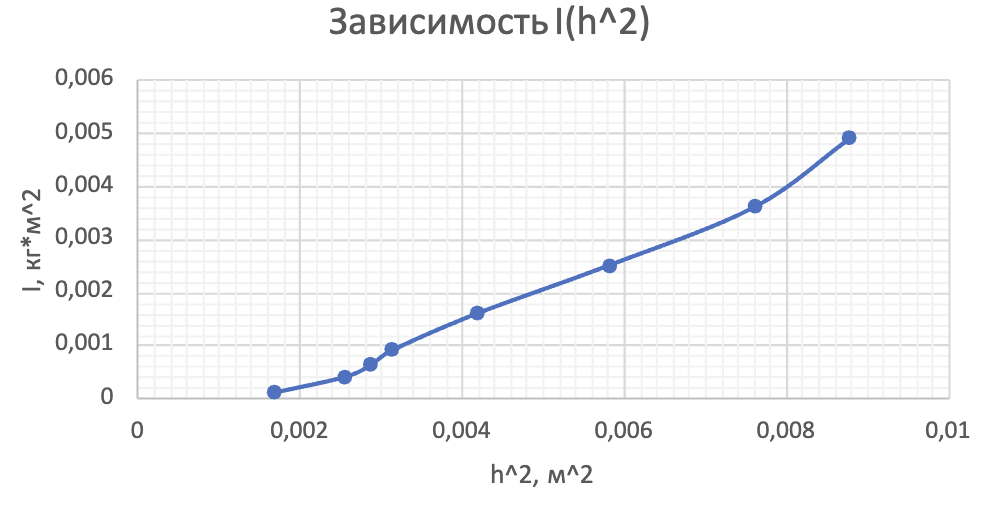
\includegraphics[scale=1]{Гр1}}
\label{fig:image}
\end{figure}

С помощью метода наименьших квадратов найдем массу системы тел и сравним ее со значением, полученным с помощью весов:

\

\begin{tabular}{lll}
                           & Эксперимент   & Теория        \\
m, г                       & $1536,5\pm0,5 $   & $1516\pm54$       \\
$I, кг\cdot м^2$ & $0,0015\pm0,0001$ & $0,0017\pm0,0001$
\end{tabular}

\

Из таблицы видно, что результаты эксперемента согласуются с теоретическими вычислениями.

\section{Выводы}
	\begin{enumerate}
		\item Величину момента инерции можно определить с помощью трифилярного подвеса. Результаты такого измерения совпадут с теоретическими предсказаниями в рамках погрешности. Довольно большая точность результатов при помощи подвеса обеспечивается малой погрешностью измерения времени, а также выбором условий, при которых крутильные колебания подвеса можно считать слабозатухающими.
		\item В ходе эксперимента была подтверждена аддитивность момента инерции. А также была еще раз проверена теорема Гюйгенса-Штейнера.
	\end{enumerate}


\end{document}

